\label{sec:install}
\subsection{Set up you board and install SDK}

\subsubsection{Connect the board}
The development board connects to a PC through USB. The first time you plug in the board, the drivers should be automatically downloaded and installed.if the drivers are not installed automatically, right-click on the device name in Device Manager and select Update driver. Alternatively, you can download the drivers \hyperlink{https://www.ftdichip.com/Drivers/VCP.htm}{FTDI}. Choose the driver that matches your Windows installation (32- or 64-bit).

To verify installation, open Device Manager. You should be able to see three USB Serial Ports. The numbers on your COM ports may be different from those in the figure.
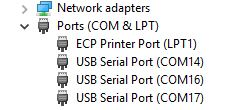
\includegraphics{COMPorts.JPG}

\subsubsection{Install the Azure Sphere SDK Preview for Visual Studio}
Azure\_Sphere\_SDK\_Preview\_for\_Visual\_Studio.exe installs the complete Azure Sphere software development kit (SDK).

To install the SDK:
\begin{enumerate}
    \item \hyperlink{https://aka.ms/AzureSphereSDKDownload}{Download the Azure Sphere SDK Preview for Visual Studio} from Visual Studio Marketplace if you have not already done so. Save the downloaded file on your PC.
    \item Run Azure\_Sphere\_SDK\_Preview\_for\_Visual\_Studio.exe from the download to install the SDK. Agree to the license terms and select Next.
    \begin{figure}[h]
    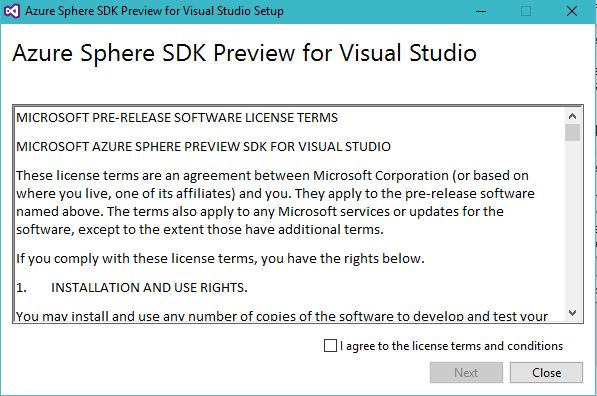
\includegraphics[scale=0.7]{SDK1.JPG}
    \end{figure}
    \newpage
    \item Click Install to begin installation.
    \begin{figure}[h]
    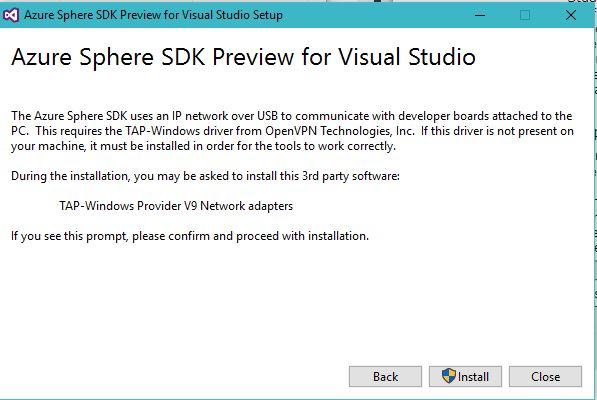
\includegraphics[scale=0.7]{SDK2.JPG}
    \end{figure}
    \newline
    If the message "This product requires Visual Studio 2017, Version 15.7 or newer" appears, ensure that Visual Studio 2017 version 15.7 or more recent is installed on your PC.

    The message "No product to install SDK on" may appear if you do not have Visual Studio version 15.7 or newer installed, or if you have just installed Visual Studio for the first time. If you see this message, either update your Visual Studio installation if necessary or restart your PC and return to this step.
    \item Accept the elevation prompt if one appears.
    \item When setup completes, restart your PC if the setup application requests it. The SDK is installed to all compatible editions of Visual Studio on your PC. The SDK requires Visual Studio version 15.7 or later.
    
\end{enumerate}

\subsection{Update OS}
If the Azure Sphere device has never been used, it most likely needs to update the OS. Follow the steps to update the Azure Sphere OS.
\begin{enumerate}
    \item Connect the board to the PC by USB.
    \item Open an Azure Sphere Developer Command Prompt. It appears in the Start menu under Azure Sphere.
    \item Issue the following command to update the Azure Sphere OS:
        \begin{lstlisting}[language=bash]
            azsphere device recover
        \end{lstlisting}
    You should see output similar to this:
        \begin{lstlisting}[language=bash]
            Starting device recovery. Please note that this may take up to 10 minutes.
            Board found. Sending recovery bootloader.
            Erasing flash.
            Sending images.
            Sending image 1 of 16.
            Sending image 2 of 16.
            . . . 
            Sending image 16 of 16.
            Finished writing images; rebooting board.
            Device ID: <GUID>
            Device recovered successfully.
            Command completed successfully in 00:02:37.3011134.
        \end{lstlisting}
\end{enumerate}

\subsubsection{Set up an account for Azure Sphere}
Azure Sphere uses Azure Active Directory (AAD) to enforce enterprise access control. Therefore, to use Azure Sphere, you need a Microsoft work or school account (sometimes called an organizational account) that is associated with an AAD.

The ÅF account is Microsoft work account, to find out you can use the account, open an Azure Sphere Developer Command prompt (on the Start menu under Azure Sphere) and sign in to Azure Sphere with your work or school account:
\begin{lstlisting}[language=bash]
    azsphere login
\end{lstlisting}
In response, azsphere prompts you to pick an account. Choose the ÅF account and type your password if required. If you see a dialog box requesting that an admin grant permission to use the Azure Sphere Utility, you'll need to log in as an administrator or obtain admin approval.

If login succeeds, the command returns a list of the Azure Sphere tenants that are available for you. You should see the similar output to this:
\begin{lstlisting}[language=bash]
    The selected Azure Sphere tenant 'AFTechnology' (4679af44-ad27-4c1d-9ef8-4f76b540edae) will be retained.
Successfully logged in with the selected AAD user. This authentication will be used for subsequent commands.
Command completed successfully in 00:00:15.3946315.
\end{lstlisting}

For more information please visit the Microsoft document on \hyperlink{https://docs.microsoft.com/en-us/azure-sphere/install/azure-directory-account}{Set up an account}.

\subsection{Claim Device}
Every device must be "claimed" by an Azure Sphere tenant. Claiming the device associates its unique, immutable device ID with your Azure Sphere tenant. The Azure Sphere Security Service uses the device ID to identify and authenticate the device.

We recommend that each company or organization create only one Azure Sphere tenant.

\begin{tcolorbox}
\textsc{\textbf{Important}\newline\newline Claiming is a one-time operation that you cannot undo even if the device is sold or transferred to another person or organization. A device can be claimed only once. Once claimed, the device is permanently associated with the Azure Sphere tenant.\newline\newline Before you claim your device, complete these steps to ensure that you use the right work/school account to create and access your Azure Sphere tenant. Your device must be connected to your PC before you create the tenant, and you can only use the device to create a single tenant.}
\end{tcolorbox}

To claim your device:
\begin{enumerate}
    \item Connect your device to your PC.
    \item Open an Azure Sphere Developer Command Prompt, which is available in the Start menu under Azure Sphere.
    \item Claim your device. After you claim your device into a tenant, you cannot move it to a different tenant.
    \begin{lstlisting}[language=bash]
    azsphere device claim
    \end{lstlisting}
    You should see the similar output like this:
    \begin{lstlisting}[language=bash]
    Claiming device.
    Successfully claimed device ID 'B3E012CE682BA0A6235866AB3A87D838A4817E5C539832A34BF7A715CA8D015FF99C84B909CB2886916259AD186B212E148FC9C4B
    F8BB6A275A11A2B9495D578' into tenant 'AFTechnology' with ID '4679af44-ad27-4c1d-9ef8-4f76b540edae'. 
    Command completed successfully in 00:00:03.4394424.
    \end{lstlisting}
\end{enumerate}

\newpage

\subsection{Configure Wi-Fi}
Before you can configure Wi-Fi, you must:
\begin{itemize}
    \item Install the SDK and set up the development board
    \item Update the OS
    \item Claim the device
\end{itemize}
Follow these steps to configure Wi-Fi on your Azure Sphere device:
\begin{enumerate}
    \item Connect your Azure Sphere board to your PC over USB.
    \item Open an Azure Sphere Developer Command Prompt.

    \item Register the device's MAC address if your network environment requires it. Use the following command to get the MAC address:
    \begin{lstlisting}[language=bash]
    azsphere device wifi show-status
    \end{lstlisting}
    \item Add your Wi-Fi network to the device by using the azsphere device wifi add command as follows:
    \begin{lstlisting}[language=bash]
    azsphere device wifi add --ssid <yourSSID> --key <yourNetworkKey>
    \end{lstlisting}
    
    Replace <yourSSID> with the name of your network and <yourNetworkKey> with your WPA/WPA2 key. Azure Sphere devices do not support WEP. Network SSIDs are case-sensitive. 

    To add an open network, omit the --key flag.

    If your network SSID or key has embedded spaces, enclose the SSID or key in quotation marks. If the SSID or key includes a quotation mark, use a backslash to escape the quotation mark. Backslashes do not require escape if they are part of a value.
    
    \begin{lstlisting}[language=bash]
    azsphere device wifi add --ssid "New SSID" --key "key \"value\" with quotes"
    \end{lstlisting}
    
    It typically takes several seconds for networking to be ready on the board, but might take longer, depending on your network environment.

    \item Use the azsphere device wifi show-status command to check the status of the connection. During update, the azsphere device wifi show-status command may temporarily show an unknown configuration state. 
    \begin{lstlisting}[language=bash]
    azsphere device wifi show-status
    
    SSID                : azureTest
    Configuration state : enabled
    Connection state    : connected
    Security state      : psk
    Frequency           : 5180
    Mode                : station
    Key management      : WPA2-PSK
    WPA State           : COMPLETED
    IP Address          : 172.28.22.2
    MAC Address         : 2c:f7:f1:08:72:df

    Command completed successfully in 00:00:01.3747119.
    \end{lstlisting}
\end{enumerate}


